\documentclass[a4paper]{amsproc}
\usepackage{amssymb}
\usepackage{amsmath}
\usepackage{graphicx}
\usepackage[hyphens]{url} \urlstyle{same}
\usepackage{float}
\usepackage{multicol}
\usepackage{caption}
\usepackage{geometry}
\newgeometry{margin=1.5in, bottom=1in}

%\usepackage[dvips]{graphicx} %% Package for inserting illustrations/figures
\theoremstyle{plain}
\newtheorem{thm}{Theorem}[section]
\newtheorem{prop}{Proposition}[section]
\newtheorem{lem}{Lemma}[section]
\newtheorem{cor}{Corollary}[section]
\theoremstyle{definition}
\newtheorem{exm}{Example}[section]
\newtheorem{dfn}{Definition}[section]
\theoremstyle{remark}
\newtheorem{rem}{Remark}[section]
\numberwithin{equation}{section}
\newtheorem{theorem}{Theorem}

%% Please, do not change the following four lines:
\renewcommand{\le}{\leqslant}\renewcommand{\leq}{\leqslant}
\renewcommand{\ge}{\geqslant}\renewcommand{\geq}{\geqslant}
\renewcommand{\setminus}{\smallsetminus}
%\setlength{\textwidth}{28cc} \setlength{\textheight}{42cc}

\title[From Markov Switching to Change Points, and Back]{From Markov Switching to Change Points, and Back}

\subjclass[2019]{}
\keywords{Markov Switching, Change Points, MCMC}

\author[Goolish]{\bfseries Ethan Goolish}
\address{ 
	Department of Statistical Science \\ 
	Cornell University   \\ 
	Ithaca\\
	New York\\
	14853}
\email{efg36@cornell.edu}


\begin{document}
	\vspace{18mm} \setcounter{page}{1} \thispagestyle{empty}
	
	\
	\maketitle
%	\section*{Abstract}
%	Enter Abstract
%	
%	\section{Introduction}
%	Enter Summary
	
	\section{Markov Chain Time Series}
	Let $X$ be a Markov Chain with $k$ states: $S_1, ..., S_k$. It is known that we can associate with $X$ a $(k \times k)$ transition matrix $P$ such that given $X_t = S_i$ (meaning chain $X$ is in state $i$ at time $t$), we have that $P_{ij}$ denotes the probability that $X_{t+1} = S_j$. However, if at time $t$, the state of $X_t$ is not directly observable, but rather $X_t$ emits some signal $y_t$ that probabilistically depends upon the (unobservable) state of $X_t$, we call $X$ a Hidden Markov Model. This is the case that will we will concern ourselves with first. In specific, we associate with each state $S_i$ a mean $\mu_i$ along with a fixed variance $\sigma^2$ so that if our chain is in state $S_i$ at time $t$, we can model our emitted signal as $y_t = \mu_i + \epsilon$, where $\epsilon \overset{i.i.d.}{\sim} N(0, \sigma^2)$. With this, we have our Markov Chain Time Series model: Begin in a state $S_1$. Using our above signal model, we obtain signal $y_1 = \mu_1 + \epsilon$. Then, we transition to a new state $S_j$ with probability $P_{1j}$. We obtain our next signal $y_2 = \mu_j + \epsilon$ before transitioning to our next state $S_{j'}$ with probability $P_{jj'}$, and so forth. Thus given a $(k \times k)$ transition matrix $P$, a $(k \times 1)$ vector of state means $S$, and a variation $\sigma^2$, we can create a time series $Y = (y_1, y_2, ..., y_n)$ of length $n$. Our question is this: given a time series created in the above manner but with unknown parameters $P$ and $S$, can we recover our transition probabilities and means? 
	
	\section{Process}
	To do so, we suggest the follow procedure. In the basic case, we will assume the number of states $k$ is known. Recall all we are given is a time series $Y = (y_1, ..., y_n)$ of length $n$ where each $y_i$ has associated with it some unknown state $S_j$, and is drawn probabilistically as $y_i = \mu_j + \epsilon$. For example, for if we took $k = 3$ and the following parameters:
	\[
	S = \begin{bmatrix} 5 & 0 & -5 \end{bmatrix}
	\qquad
	\sigma^2 = 1
	\qquad
	P = \begin{pmatrix} 
	0.95 & 0.02 & 0.03 \\
	0.01 & 0.95 & 0.04 \\
	0.03 & 0.03 & 0.94 \\
	\end{pmatrix}
	\]
	we could have the following series:\\
    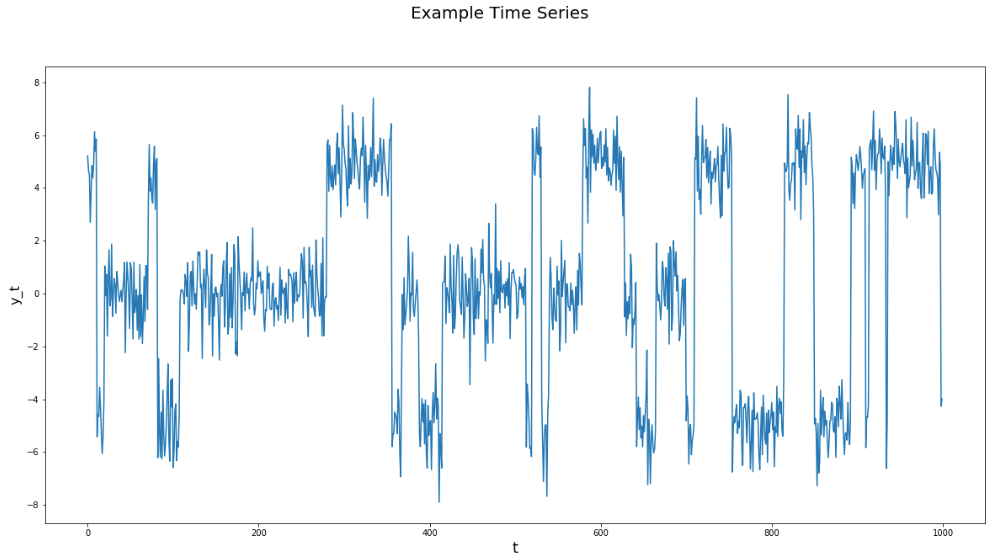
\includegraphics[scale=0.4]{examplets.png}\\
    Our suggested method takes advantage of the ECP change point package (TODO: cite). Within this package, we can use the $e\_divisive$ call to divide a time series $Y$ into segments based on its change points. The method takes several parameters including $Y$, the time series in question, $k$, the number of estimated change points, $alpha$, the exponentiation for the distance matrix, and $min\_size$, the minimum number of points allowed between change point estimations. For our method, we want to overpredict the number of change points to ensure all change points between one state $S_i$ and another state $S_j$ are found, and then merge the extraneous splits that separate two segments that should belong to the same state. Currently, we estimate $k$ by assuming the transition probabilities to be no lower than $0.75$, thus assuming the average time before transition to be approximately $1/(1 - 0.75) = 4$. Then we take $n/4$, where $n$ is the total length of $Y$, to be a rough approximation of the number of change points, and then add $n/100$ more in order to over-estimate $k$ appropriately. We also take $alpha$ to be $2$, and take $min\_size$ to be the smallest allowed ($2$) to allowed for the finest granularity. With this set of parameters, we expect a call to $e\_divisive$ to return segmentation similar to the following:\\
    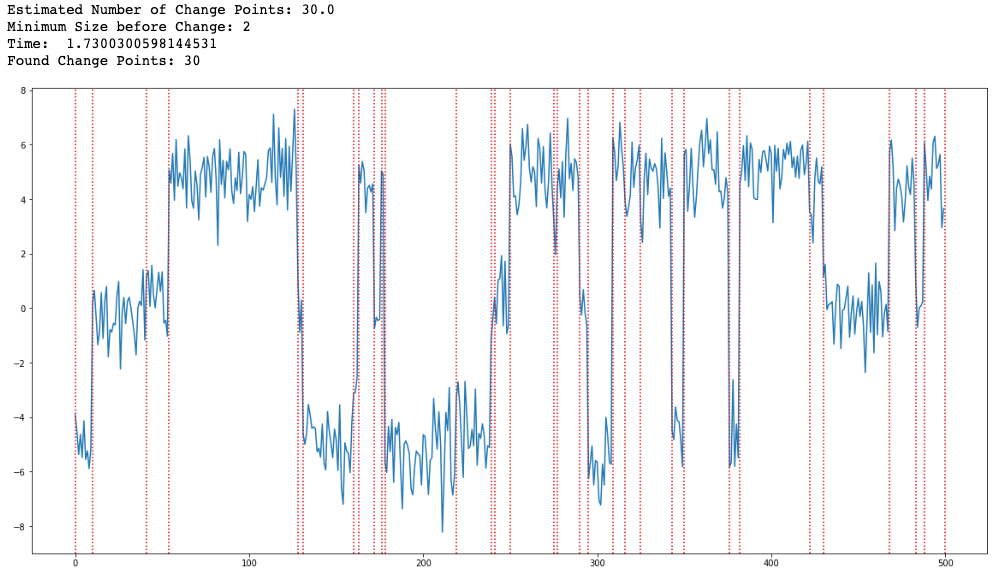
\includegraphics[scale=0.4]{examplesplit.png}\\
    Note for the most part that while the state transitions are marked by $e\_divisive$, we have some excess segmentation, such as the third mark which incorrectly divides two segments from the same state $S_1$, the state corresponding to $\mu_1 = 0$. Our next goal is to remove such incorrect splitting. To do this, begin by finding the mean $g_i$ of each guessed segment $G_i$ (which was returned by $e\_divisive$). Then, sort the list of $G_i$ incrementally by their respective $g_i$. We can then run $e\_divisive$ for a second time on our sorted $G_i$ to group our means into estimates for which state each segment guess was in. In other words, using $e\_divisive$ on a sorted list of $g_i$ groups each $G_i$ into a guess for the segment label $\hat{S_i}$. If the number of states $k$ is known, we can use $k - 1$ as the parameter for the number of change points in this second use of $e\_divisive$. To continue the above example, here we plot the sorted means $g_i$, and then segment using the second $e\_divisive$ call. The segments $G_i$ corresponding to points in the first segment will be estimated to be in state $\hat{S_0}$, the segments corresponding to points in the second segment will be estimated to be in state $\hat{S_1}$, and the segments corresponding to points in the third segment will be estimated to be in state $\hat{S_2}$:\\
    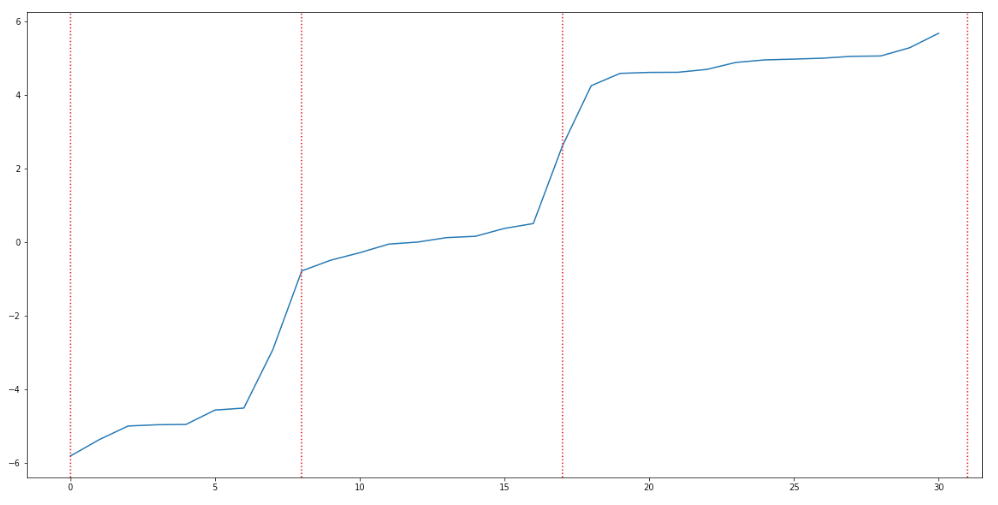
\includegraphics[scale=0.4]{example2x.png}\\
    After assigning each $G_i$ to the appropriate $\hat{S_i}$, we then do the merging -- we can iterate through our original (unsorted) list of $G_i$, and if some $G_i$ and $G_{i+1}$ have the same assigned state label $\hat{S_i}$, then we propose a new segment $G_i'$ such that $G_i'$ contains the points that used to be in $G_i$ and $G_{i+1}$. After doing this, we get this new estimation of the change points, which we can see is much more accurate:\\
    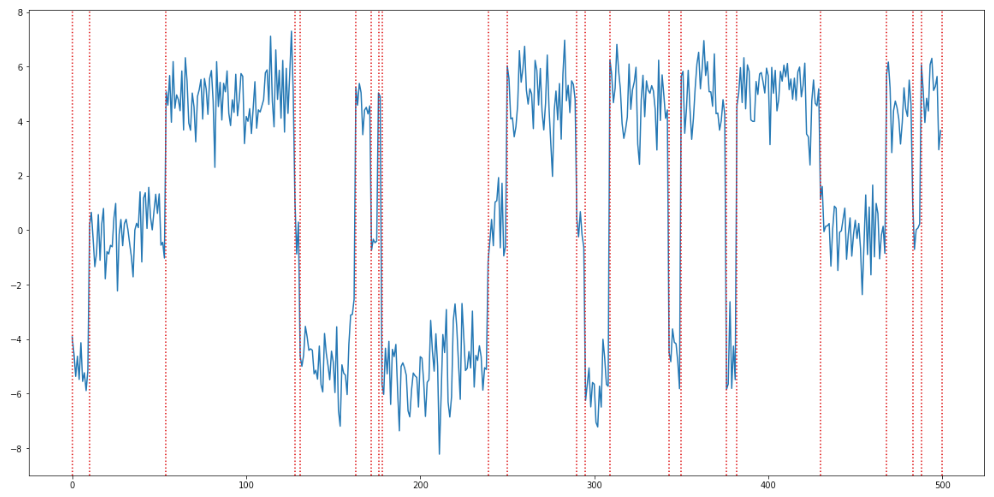
\includegraphics[scale=0.4]{examplefixedseg.png}\\
    Now with our fixed segmentation, we estimate our transition probabilities $P_{i, j}$ as well as our state means $\mu_i$. To do so, we first calculate the average stay time for each state label $\hat{S_i}$. By this we mean we take each updated segment $G_i$ and observe its length. We groupby the segment labels $\hat{S_i}$ and take the average to find the average time of stay for a given label $\hat{S_i}$, call it $a_i$. Then note that
    \[
    a_i = \frac{1}{1 - P_{i, i}} \iff P_{i, i} = \frac{a_i - 1}{a_i}
    \] 
    and thus we can estimate our staying probabilities $P_{i, i}$. We can also estimate our off-diagonal probabilities $P_{i, j}$: We first count the number of times we transition from a state $i$ to every other state $j$ where $j \neq i$, call it $c_{i, j}$. Then, we know that $P_{i, j}$ is proportional to the number of times we transition from $i$ to $j$ over the number of times we transition from $i$ to any other state $j'$. Since we know the sum across a row $\sum_j P_{i, j} = 1$, we can say
    \[
    P_{i, j} = \frac{c_{i, j}(1 - P_{i, i})}{\sum_j c_{i, j}}
    \]
    Alternatively, we can take a prior $\alpha_i$ so that $c'_{i, j} = c_{i, j} + \alpha_i$. In this basic example we take $\alpha_i = 0$, but other natural choices include $\alpha_i = 1$, $\alpha_i = 1/2$, or $\alpha_i = 1/K$ (where $K$ is our number of states). In total, this gives us our full probability matrix $P$.\\ 
    
    Then, to estimate $S = \{\mu_1, ...., \mu_k\}$, we simply groupby our updated segment labels $\hat{S_i}$ and take the mean to find each $\hat{\mu_i}$. Doing the above on our example dataset above yields us:
    \[
    \hat{S} = \begin{bmatrix} -5.04134908 & -0.03278774 & 4.91458622 \end{bmatrix}
    \qquad
    \hat{P} = \begin{pmatrix} 
    0.95384615 & 0.01538462 & 0.03076923 \\
    0.01818182 & 0.93636364 & 0.04545455 \\
    0.01298077 & 0.02163462 & 0.96538462 \\
    \end{pmatrix}
    \]
	yielding us an accurate recovering of our original parameters.\\
    
\end{document}